%Version 3.1 December 2024
% See section 11 of the User Manual for version history
%
%%%%%%%%%%%%%%%%%%%%%%%%%%%%%%%%%%%%%%%%%%%%%%%%%%%%%%%%%%%%%%%%%%%%%%
%%                                                                 %%
%% Please do not use \input{...} to include other tex files.       %%
%% Submit your LaTeX manuscript as one .tex document.              %%
%%                                                                 %%
%% All additional figures and files should be attached             %%
%% separately and not embedded in the \TeX\ document itself.       %%
%%                                                                 %%
%%%%%%%%%%%%%%%%%%%%%%%%%%%%%%%%%%%%%%%%%%%%%%%%%%%%%%%%%%%%%%%%%%%%%

%%\documentclass[referee,sn-basic]{sn-jnl}% referee option is meant for double line spacing

%%=======================================================%%
%% to print line numbers in the margin use lineno option %%
%%=======================================================%%

%%\documentclass[lineno,pdflatex,sn-basic]{sn-jnl}% Basic Springer Nature Reference Style/Chemistry Reference Style

%%=========================================================================================%%
%% the documentclass is set to pdflatex as default. You can delete it if not appropriate.  %%
%%=========================================================================================%%

%%\documentclass[sn-basic]{sn-jnl}% Basic Springer Nature Reference Style/Chemistry Reference Style

%%Note: the following reference styles support Namedate and Numbered referencing. By default the style follows the most common style. To switch between the options you can add or remove “Numbered” in the optional parenthesis. 
%%The option is available for: sn-basic.bst, sn-chicago.bst%  
 
%%\documentclass[pdflatex,sn-nature]{sn-jnl}% Style for submissions to Nature Portfolio journals
%%\documentclass[pdflatex,sn-basic]{sn-jnl}% Basic Springer Nature Reference Style/Chemistry Reference Style
\documentclass[pdflatex,sn-mathphys-num]{sn-jnl}% Math and Physical Sciences Numbered Reference Style
%%\documentclass[pdflatex,sn-mathphys-ay]{sn-jnl}% Math and Physical Sciences Author Year Reference Style
%%\documentclass[pdflatex,sn-aps]{sn-jnl}% American Physical Society (APS) Reference Style
%%\documentclass[pdflatex,sn-vancouver-num]{sn-jnl}% Vancouver Numbered Reference Style
%%\documentclass[pdflatex,sn-vancouver-ay]{sn-jnl}% Vancouver Author Year Reference Style
%%\documentclass[pdflatex,sn-apa]{sn-jnl}% APA Reference Style
%%\documentclass[pdflatex,sn-chicago]{sn-jnl}% Chicago-based Humanities Reference Style

%%%% Standard Packages
%%<additional latex packages if required can be included here>

\usepackage{graphicx}%
\usepackage{multirow}%
\usepackage{amsmath,amssymb,amsfonts}%
\usepackage{amsthm}%
\usepackage{mathrsfs}%
\usepackage[title]{appendix}%
\usepackage{xcolor}%
\usepackage{textcomp}%
\usepackage{manyfoot}%
\usepackage{booktabs}%
\usepackage{algorithm}%
\usepackage{algorithmicx}%
\usepackage{algpseudocode}%
\usepackage{listings}%
%%%%

%%%%%=============================================================================%%%%
%%%%  Remarks: This template is provided to aid authors with the preparation
%%%%  of original research articles intended for submission to journals published 
%%%%  by Springer Nature. The guidance has been prepared in partnership with 
%%%%  production teams to conform to Springer Nature technical requirements. 
%%%%  Editorial and presentation requirements differ among journal portfolios and 
%%%%  research disciplines. You may find sections in this template are irrelevant 
%%%%  to your work and are empowered to omit any such section if allowed by the 
%%%%  journal you intend to submit to. The submission guidelines and policies 
%%%%  of the journal take precedence. A detailed User Manual is available in the 
%%%%  template package for technical guidance.
%%%%%=============================================================================%%%%

%% as per the requirement new theorem styles can be included as shown below
\theoremstyle{thmstyleone}%
\newtheorem{theorem}{Theorem}%  meant for continuous numbers
%%\newtheorem{theorem}{Theorem}[section]% meant for sectionwise numbers
%% optional argument [theorem] produces theorem numbering sequence instead of independent numbers for Proposition
\newtheorem{proposition}[theorem]{Proposition}% 
%%\newtheorem{proposition}{Proposition}% to get separate numbers for theorem and proposition etc.

\theoremstyle{thmstyletwo}%
\newtheorem{example}{Example}%
\newtheorem{remark}{Remark}%

\theoremstyle{thmstylethree}%
\newtheorem{definition}{Definition}%

\raggedbottom
%%\unnumbered% uncomment this for unnumbered level heads

\begin{document}

\title[Map-STDP]{Map-STDP: Does it form cortices?}

%%=============================================================%%
%% GivenName	-> \fnm{Joergen W.}
%% Particle	-> \spfx{van der} -> surname prefix
%% FamilyName	-> \sur{Ploeg}
%% Suffix	-> \sfx{IV}
%% \author*[1,2]{\fnm{Joergen W.} \spfx{van der} \sur{Ploeg} 
%%  \sfx{IV}}\email{iauthor@gmail.com}
%%=============================================================%%

\author{\fnm{Vikram} \sur{Ramavarapu}}
% \email{vikramr2@illinois.edu}

% \affil[1]{\orgdiv{Computer Science}, \orgname{University of Illinois}, \orgaddress{\city{Urbana}, \state{Illinois}, \country{USA}}}
%%==================================%%
%% Sample for unstructured abstract %%
%%==================================%%

\abstract{STDP is a local learning rule that may not capture the global modular structure of the neural network. In this paper, a new Map-STDP rule is derived using the map equation, which is an info-theoretic objective function for community detection.}

%%================================%%
%% Sample for structured abstract %%
%%================================%%

% \abstract{\textbf{Purpose:} The abstract serves both as a general introduction to the topic and as a brief, non-technical summary of the main results and their implications. The abstract must not include subheadings (unless expressly permitted in the journal's Instructions to Authors), equations or citations. As a guide the abstract should not exceed 200 words. Most journals do not set a hard limit however authors are advised to check the author instructions for the journal they are submitting to.
% 
% \textbf{Methods:} The abstract serves both as a general introduction to the topic and as a brief, non-technical summary of the main results and their implications. The abstract must not include subheadings (unless expressly permitted in the journal's Instructions to Authors), equations or citations. As a guide the abstract should not exceed 200 words. Most journals do not set a hard limit however authors are advised to check the author instructions for the journal they are submitting to.
% 
% \textbf{Results:} The abstract serves both as a general introduction to the topic and as a brief, non-technical summary of the main results and their implications. The abstract must not include subheadings (unless expressly permitted in the journal's Instructions to Authors), equations or citations. As a guide the abstract should not exceed 200 words. Most journals do not set a hard limit however authors are advised to check the author instructions for the journal they are submitting to.
% 
% \textbf{Conclusion:} The abstract serves both as a general introduction to the topic and as a brief, non-technical summary of the main results and their implications. The abstract must not include subheadings (unless expressly permitted in the journal's Instructions to Authors), equations or citations. As a guide the abstract should not exceed 200 words. Most journals do not set a hard limit however authors are advised to check the author instructions for the journal they are submitting to.}

% \keywords{keyword1, Keyword2, Keyword3, Keyword4}

%%\pacs[JEL Classification]{D8, H51}

%%\pacs[MSC Classification]{35A01, 65L10, 65L12, 65L20, 65L70}

\maketitle

\section{Introduction}\label{sec1}

\subsection{Problem}
Spike-timing dependent plasticity (STDP) \cite{Shouval2010-uj} is a biologically plausible learning rule that has been widely used in spiking neural networks. When a pre-synaptic neuron fires shortly before a post-synaptic neuron, the synapse between them is strengthened. Conversely, if the pre-synaptic neuron fires shortly after the post-synaptic neuron, the synapse is weakened.

However, STDP is a fully local rule that may not capture the global structure of the neural network. Ideally, we want our learning rule to guide our network to form \emph{cortices}, which are densely connected communities of neurons that are sparsely connected to other communities.

\subsection{Why Cortices?}

Cortices enable expressive spatial population codes that can perform representations such that cortices can be mapped to concepts.

For example, in the case of ImageNet classification, we want the network to learn a modular structure where each community corresponds to a different class. This would allow the network to learn a more efficient representation of the data, as it would be able to leverage the modular structure to learn more compact representations of each class.

In the case of the Gymnasium car racing environment, we would want the network to form five cortices that correspond to: do nothing, accelerate, brake, turn left, and turn right.

\subsection{Random Walks and the Map Equation}

Neural dynamics are very stochastic and operate as a form of random walk \cite{Buesing2011-ka}, which is a major component of the map equation, an info-theoretic objective function for community detection in the Infomap algorithm \cite{Rosvall2008-vf}. The map equation measures the modular structure of a network by quantifying the amount of information needed to describe the flow of activity through the network via a random walk.

As such, a Map-STDP rule that incorporates the map equation is derived. The Map-STDP rule is a local learning rule that can capture the global modular structure of the neural network. Moreover, the Map-STDP rule preserves biorealism through the use of info-theoretic entropy maximization, stochastic neural dynamics, and local synaptic updates.

\section{Infomap and Entropy}

\subsection{Infomap}

The Infomap algorithm is a community detection algorithm that minimizes the map equation to identify communities in a network. The map equation is defined as:

$$L(M) = q_{\curvearrowright} H(\mathcal{Q}) + \sum_{m \in M} p_{\circlearrowright}^{m} H(\mathcal{P}^{m})$$

where $M$ is a partition of the network into $m$ communities. There are two terms. The first term represents the entropy of movement between communities, will the second term represents the entropy of movement within communities, where exiting the community is also considered a movement.

\subsection{Connecting the Map Equation to Neural Computation}

Map-STDP is designed to be compounded with a standard STDP rule that maximizes mutual information between stimulus and neural response, a well-established consequence of Hebbian learning under information-theoretic objectives \cite{dayan2001information}. The STDP term handles single-neuron expressivity, while the map equation term acts as a structural constraint at the population level.

The deeper grounding comes from variational free energy \cite{Friston2010-cj}. The SNN's MCMC dynamics \cite{Buesing2011-ka} produce a stationary distribution $p(\mathbf{z}|\mathbf{o})$ over neural activity patterns given sensory input $\mathbf{o}$. This is precisely the recognition density that minimizes variational free energy. This distribution represents the network's implicit model of the world. The map equation operates on the marginal visit frequencies $\tilde{p}_i = p(z_i = 1 | \mathbf{o})$, which are byproducts of this same sampling process. Map-STDP therefore does not introduce a separate objective: it imposes community structure on the distribution the network is already converging to, with the addition of mesoscale organization of $p(\mathbf{z}|\mathbf{o})$.

\section{Deriving Map-STDP}\label{sec2}

As mentioned earlier, in order to properly address response entropy, the Map-STDP rule should be compounded with an STDP rule that maximizes response entropy. As such, we can start with a rule in the form of:

\begin{equation}
\Delta W_{ij} = \eta \cdot \text{STDP}(i, j) - \eta' \cdot G(i, j)
\label{eq:learning-rate}
\end{equation}

where $\text{STDP}(i, j)$ is a standard STDP rule that maximizes response entropy, $G(i, j)$ is a modular gating function, and $\eta$, $\eta'$ are separate learning rates for the two objectives. The two terms are additive rather than multiplicative, so each objective acts independently: STDP drives the synaptic updates toward maximizing response entropy, while the map gradient term descends the map equation loss to encourage modular structure. The goal is to derive the form of $G(i, j)$.

In its general form, a random walk on a network has a transition matrix $T$ that can be defined as:

$$T_{ij} = \frac{W_{ij}}{\sum_k W_{ik}}$$

where $W_{ij}$ is the weight of the edge from node $i$ to node $j$. We can then tie this in to Buesing et. al.'s equation for the membrane potential of a neuron in an SNN that performs MCMC sampling \cite{Buesing2011-ka}:

$$u_i = b_i + \sum_j W_{ij} z_j(t)$$

where $u_i$ is the membrane potential of neuron $i$, $b_i$ is the bias of neuron $i$, and $z_j(t)$ is the binary spike variable of neuron $j$ at time $t$. While $z$ is an instantaneous variable, we can take its expectation over time in order to make it compatible with the map equation's flow-based framework. This gives us:

$$\langle z_j \rangle = \tilde{p}_j = p(z_j = 1 | \mathbf{o})$$

This gives us the corrected definition of our transition matrix as:

$$\tilde{T}_{ij} = \frac{W_{ij} \tilde{p}_j}{\sum_k W_{ik} \tilde{p}_k} = \frac{\tilde{W}_{ij}}{\tilde{s}_i}$$

With our new defined variables $\tilde{W}_{ij} = W_{ij} \tilde{p}_j$ and $\tilde{s}_i = \sum_k W_{ik} \tilde{p}_k$.

The Chapman-Kolmogorov equation then gives us the probability of being at node $j$ at time $t$ as:

$$\pi_j^{t+1} = \sum_i \tilde{T}_{ij}\pi_i^t$$

The stationary distribution therefore satisfies:

$$\tilde{p}_j = \sum_i \tilde{T}_{ij} \tilde{p}_i\rightarrow \tilde{p} = \tilde{T} \tilde{p}$$

We can rule out the trivial solution of $\tilde{p} = 0$ by enforcing a normalization constraint of $\sum_j \tilde{p}_j = 1$. Another trivial solution we can rule out is the one where $\tilde{T}=I$, which could only be true if we don't add a constraint of irreducibility, meaning there must be some level of connectivity between all nodes in the network. This is then reducible to a fixed point problem, therefore we can then solve for $\tilde{p}$ using power iteration:

$$\tilde{p}^{(k+1)} = \tilde{T} \tilde{p}^{(k)}$$

Which can be estimated online via the local update rule:
\begin{equation}
\tilde{p}_i \leftarrow (1-\beta) \tilde{p}_i + \beta \sum_j \tilde{T}_{ij} z_j(t)
\label{eq:local-update}
\end{equation}

It is worth noting that the stationary probability $\tilde{p}$ is also the PageRank of the network with transition matrix $\tilde{T}$. The above rule is actually a form of the iterative step of the power iteration method for computing PageRank.

The proofs of convergence are deferred to Appendix~\ref{sec:proofs}.

Now, it's time to come back to the map equation and derive the form of $G(i, j)$. We can rewrite $p_{\circlearrowright}^m$ and $q_{\curvearrowright}$ in terms of $\tilde{p}$:

$$p_m := \sum_{i \in m} \tilde{p}_i$$
$$q_m := \sum_{i \in m} \sum_{j \notin m} \tilde{T}_{ij} \tilde{p}_i$$
$$p_{\circlearrowright}^m = p_m + q_m$$
$$q_{\curvearrowright} = \sum_{m \in M} q_m$$

Where $p_m$ is the total visit frequency of community $m$, and $q_m$ is the total exit frequency of community $m$. We can then rewrite the map equation as:

$$L(M) = q_{\curvearrowright} H(\mathcal{Q}) + \sum_{m \in M} (p_m + q_m) H(\mathcal{P}^m)$$

Now we need to expand the entropy terms.

$$H(\mathcal{Q}) = -\sum_{m \in M} \frac{q_m}{q_{\curvearrowright}} \log \left( \frac{q_m}{q_{\curvearrowright}} \right)$$

$$H(\mathcal{P}^m) = -\frac{q_m}{p_m + q_m} \log \left( \frac{q_m}{p_m + q_m} \right) - \sum_{i \in m} \frac{\tilde{p}_i}{p_m + q_m} \log \left( \frac{\tilde{p}_i}{p_m + q_m} \right)$$

Now, substituting this back into the map equation gives us:

\begin{align*}
L(M) &= -\sum_{m \in M} q_m \log \left( \frac{q_m}{q_{\curvearrowright}} \right) + \sum_{m \in M} q_m \log \left( \frac{q_m}{p_m + q_m} \right) + \sum_{m \in M} \sum_{i \in m} \tilde{p}_i \log \left( \frac{\tilde{p}_i}{p_m + q_m} \right)
\end{align*}

Now we can take the gradient with respect to $W_{ij}$. The first term requires two dependent derivatives via the chain rule: $\partial q_m / \partial W_{ij}$ and $\partial q_{\curvearrowright} / \partial W_{ij}$. The second term also requires two dependent derivatives: $\partial q_m / \partial W_{ij}$ and $\partial p_m / \partial W_{ij}$. The third term requires two dependent derivatives: $\partial \tilde{p}_i / \partial W_{ij}$ and $\partial p_m / \partial W_{ij}$.

When computing $\partial \tilde{p}_i / \partial W_{ij}$:

$$\frac{\partial \tilde{p}_i}{\partial W_{ij}} = \left[\frac{\partial \tilde{T}\tilde{p}}{\partial W_{ij}}\right]_i$$
$$= \left[\frac{\partial \tilde{T}}{\partial W_{ij}} \tilde{p} + \tilde{T} \frac{\partial \tilde{p}}{\partial W_{ij}}\right]_i = \left[\frac{\partial \tilde{p}}{\partial W_{ij}}\right]_i$$

Removing the $[\cdot]_i$ operator gives us a fixed point partial differential equation. We can solve this as follows:

$$\frac{\partial \tilde{p}}{\partial W_{ij}} = (I - \tilde{T})^{-1} \frac{\partial \tilde{T}}{\partial W_{ij}} \tilde{p}$$

This raises the issue of a global matrix inversion. We sidestep it by treating $\tilde{p}$ as constant with respect to $W_{ij}$ during the synaptic update, consistent with an EM interpretation: the E-step re-estimates $\tilde{p}$ via Equation~\ref{eq:local-update}, while the M-step optimizes $W$ with $\tilde{p}$ held fixed. Under this approximation, $\partial p_m / \partial W_{ij} = 0$.

When we derive $G(i, j)$ under this approximation, we get the following form:

$$G(i, j) = \tilde{p}_i \tilde{p}_j \frac{\mathbb{I}[j \notin m(i)] \tilde{s}_i - e_i}{\tilde{s}_i^2} \log \frac{q_{\curvearrowright}}{p_{m(i)} + q_{m(i)}}$$

The full derivation can be found in Appendix~\ref{sec:proofs}.

Where $e_i = \sum_{j' \notin m(i)} W_{ij'} \tilde{p}_{j'}$ is the total exit flow from node $i$. The gating function $G(i, j)$ is the same as the gradient of the map equation with respect to $W_{ij}$, treating $\tilde{p}$ as constant with respect to $W$.

We can potentially simplify this equation by removing terms that have constant sign, assuming they get absorbed into the learning rate. For example, $\tilde{p}_i$, $\tilde{p}_j$, and $\tilde{s}_i$ are always positive, so they can be removed without affecting the direction of the update. We want to keep our network modular. This means that so long as we keep our learning rate negative (which in Equation \ref{eq:learning-rate}, we do), we can remove the log term as well, since $q_{\curvearrowright} < p_{m(i)} + q_{m(i)}$ is a necessary condition for modularity. This gives us the following simplified form of the Map-STDP rule:

\begin{equation}
G_{sim}(i, j) = \mathbb{I}[j \notin m(i)] - \frac{e_i}{\tilde{s}_i}
\end{equation}

Given a negative learning rate for the gating term, this simplified rule can be interpreted as follows: if $j \notin m(i)$, then $G_{sim}(i, j) = 1 - \bar{e}_i > 0$, so $W_{ij}$ is decreased, discouraging cross-community connectivity. If $j \in m(i)$, then $G_{sim}(i, j) = -\bar{e}_i < 0$, so $W_{ij}$ is increased, reinforcing intra-community connectivity. In both cases the magnitude of the update is modulated by $\bar{e}_i = e_i / \tilde{s}_i$, the current normalized exit probability of node $i$. This means nodes that are already well-contained within their community ($\bar{e}_i \approx 0$) receive small updates, while nodes with high community leakage ($\bar{e}_i \approx 1$) receive large corrections. The rule is self-regulating in the sense that it applies the strongest pressure where community structure is most violated.

One issue that is raised is that needing to compute $e_i$ and $\tilde{s}_i$ for every synaptic update violates locality. However, since $W_{ij}=0$ for non-neighbors, we can compute $e_i$ and $\tilde{s}_i$ using only local information from the neighbors of node $i$:
\begin{equation}
e_i = \sum_{j' \in N(i)} \mathbb{I}[j' \notin m(i)] W_{ij'} \tilde{p}_{j'}
\end{equation}

\begin{equation}
\tilde{s}_i = \sum_{k \in N(i)} W_{ik} \tilde{p}_k
\end{equation}

Where $N(i)$ is the set of neighbors of node $i$. This means that the Map-STDP rule can be implemented in a biologically plausible manner, as it only requires information from the local neighborhood of each synapse.

\section{Biological Plausibility}\label{sec11}

Earlier we touched upon the use of an STDP term alongside a Map Equation term in order to maximize response entropy while also encouraging modular structure through the minimization of free energy.

However, there are several aspects of Map-STDP that are less biologically plausible:\begin{itemize}
    \item \textbf{Community Assignments:} The Map-STDP rule requires knowledge of the community assignment of each node, which is not something that is explicitly represented in the brain.
    \item \textbf{EM Phase Separation:} The Map-STDP rule relies on an EM-like separation of timescales, where the E-step updates the stationary distribution $\tilde{p}$ while the M-step updates the weights $W$ with $\tilde{p}$ held constant. This separation may not be biologically realistic, as it requires a level of coordination and synchronization that may not be present in neural circuits.
\end{itemize}

The crux of the issue lies in the global assignment of nodes to communities. In real cortices, lateral inhibition is a local mechanism that can give rise to the emergence of distinct communities without the need for an explicit global community assignment. 

Lateral inhibition provides a local, emergent mechanism to replace the explicit community assignment $\mathbb{I}[j \notin m(i)]$. Introduce a set of inhibitory synaptic weights $\mathbf{I}$, where $I_{ij} \geq 0$ is the strength of inhibitory projection from neuron $j$ onto neuron $i$. Define the normalized inhibitory competition score:

$$\varphi_{ij} = \frac{I_{ij} \tilde{p}_j}{\sum_k I_{ik} \tilde{p}_k}$$

This $\varphi_{ij}$ is high when $j$ is a strong inhibitory competitor of $i$---which emerges when $j$ and $i$ belong to functionally distinct communities---and near zero when $j$ cooperates with $i$. Replacing $\mathbb{I}[j \notin m(i)]$ with $\varphi_{ij}$ and redefining the exit flow as $e_i^{LI} = \sum_{j'} \varphi_{ij'} W_{ij'} \tilde{p}_{j'}$ gives the laterally-inhibited gating function:

\begin{equation}
G_{LI}(i,j) = \varphi_{ij} - \bar{e}_i^{LI}
\end{equation}

where $\bar{e}_i^{LI} = e_i^{LI} / \tilde{s}_i$ is the normalized exit flow weighted by the inhibitory competition score. Under this formulation, community membership is no longer an explicit global label: it is instead encoded implicitly in the inhibitory drive, with neurons that strongly suppress one another treated as belonging to different communities.

The inhibitory weights $\mathbf{I}$ can themselves be updated via an anti-Hebbian rule: $\Delta I_{ij} = \eta_{inh} \cdot \tilde{p}_i \cdot \tilde{p}_j$, which strengthens inhibition between co-active neurons and allows competition boundaries to sharpen over time.

This formulation also clarifies what Map-STDP with lateral inhibition offers over lateral inhibition alone. Lateral inhibition by itself (as in Kohonen self-organizing maps) creates competition-driven community structure but optimizes an implicit objective---the partition that emerges is whatever the winner-take-all dynamics produce, with no guarantee of quality. Map-STDP adds two things that lateral inhibition cannot provide:

\begin{itemize}
    \item \textbf{An explicit information-theoretic objective.} The map equation gives a measurable criterion for partition quality: the description length of a random walk through the network. This makes the community structure interpretable and quantifiable, rather than an emergent side-effect.
    \item \textbf{Self-regulating update magnitude.} The term $\bar{e}_i^{LI}$ acts as adaptive gain control. Neurons already well-contained within their functional community (low $\bar{e}_i^{LI}$) receive small updates; neurons with high cross-community leakage receive large corrections. Lateral inhibition alone only suppresses competitors---it has no such signal about how far the current partition is from the optimum.
\end{itemize}

\section{Training}\label{sec12}

\begin{figure}
\centering
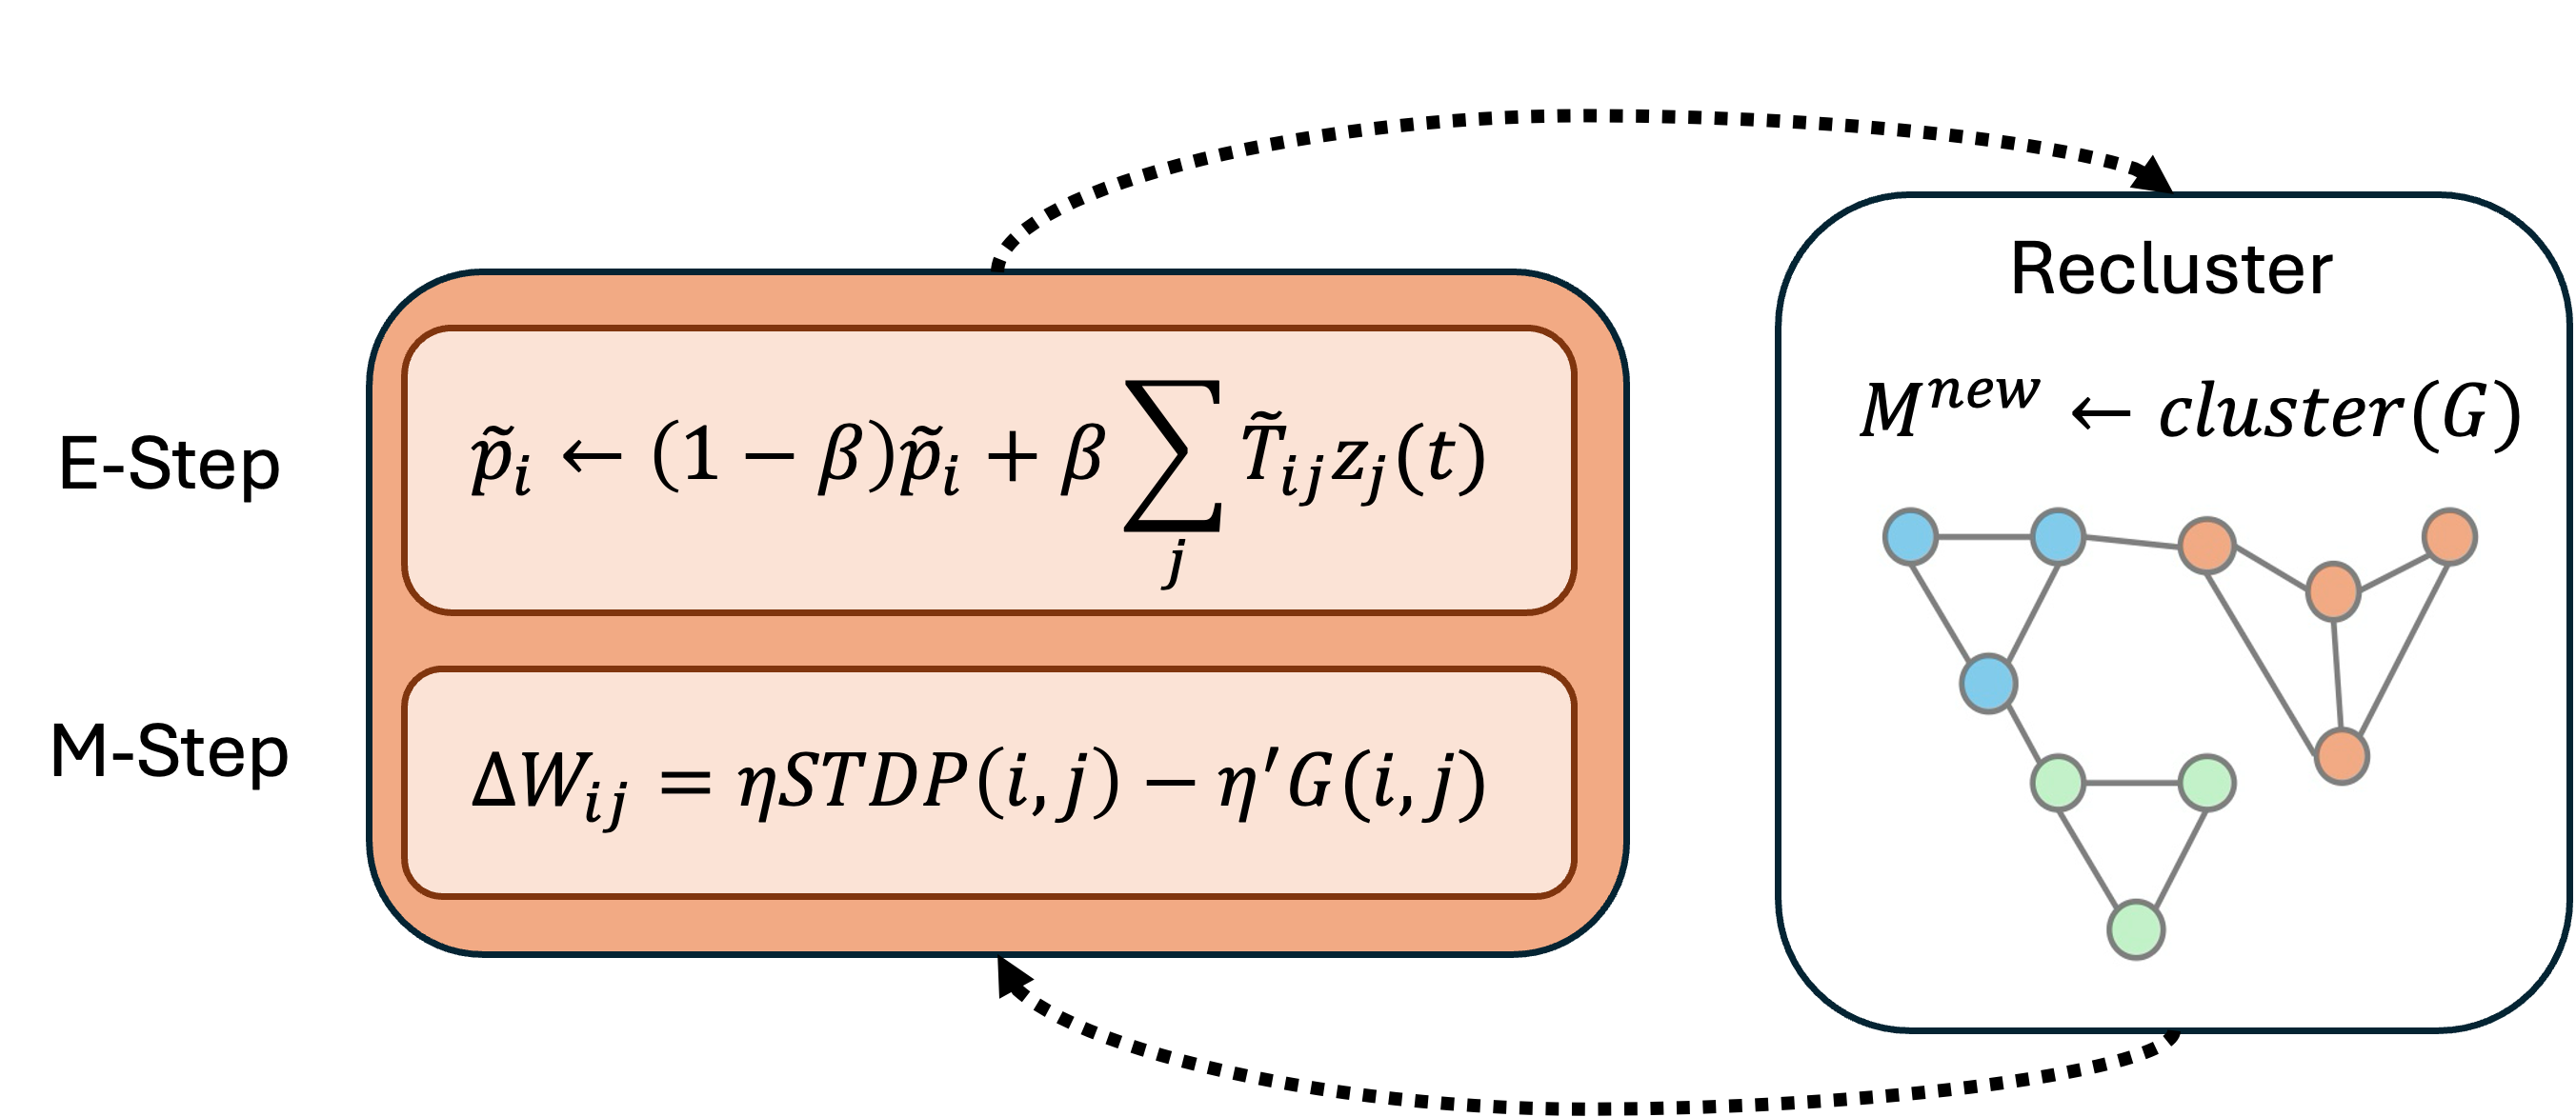
\includegraphics[width=0.8\textwidth]{algo_infograph.png}
\caption{The network of updates during training. The Map-STDP rule would involve an E-step where the network dynamics are run to update $\tilde{p}$, and an M-step where $W$ is updated using the Map-STDP rule with $\tilde{p}$ held constant. The community assignments $M$ can either be kept static or periodically updated using a community detection algorithm.}
\end{figure}

Now that we have derived the Map-STDP rule, we need to work out the mechanics of training. There are four main structures that need to be cached:

\begin{itemize}
    \item $M$: the community assignment of each node. This can be stored as a vector of integers, where the $i$-th element is the community that node $i$ belongs to.
    \item $\tilde{p}$: the stationary distribution of the random walk on the network. This can be stored as a vector of floats, where the $i$-th element is the stationary probability of node $i$.
    \item $N(i)$: the set of neighbors of each node. This can be stored as a list of lists, where the $i$-th element is a list of the neighbors of node $i$.
    \item $W$: the weight matrix of the network. This can be stored as a 2D array, where the element at row $i$ and column $j$ is the weight of the edge from node $i$ to node $j$.
\end{itemize}

With this leaves us with some open questions:

\begin{itemize}
    \item \textbf{Should $M$ be kept static or periodically updated?} If we keep $M$ static, then the Map-STDP rule will only reinforce the initial community structure, which may not be optimal. On the other hand, if we periodically update $M$ using a community detection algorithm like Infomap, then the Map-STDP rule will be able to adapt to changes in the network structure and potentially find better community assignments. However, this comes at the cost of increased computational complexity due to running a community detection algorithm at each update step.
    \item \textbf{How do we get the SNN to update its topology?} As opposed to simply just its weights. One possibility is that we set some hyperparameter $\epsilon$ such that if $W_{ij} < \epsilon$, then we set $W_{ij} = 0$. This would allow the network to prune weak connections and potentially form more distinct communities. However, this also introduces a new hyperparameter that needs to be tuned, and it may lead to instability in the training process if not handled carefully. Another possibility is a $k$ parameter such that all nodes have their top $k$ strongest connections kept and the rest set to zero. This would ensure that the network maintains a certain level of connectivity while still allowing for pruning of weaker connections. However, this also introduces a new hyperparameter that needs to be tuned, and it may lead to instability if $k$ is set too low or too high.
    \item \textbf{How do we initialize the SNN, and $M$?} One possibility is to initialize as a random Erdos-Renyi graph, with communities initialized randomly such that each node has a $1/|M|$ chance of being assigned to each community. This would provide a neutral starting point for the network to learn from, without any inherent bias towards a particular community structure. However, this also means that the network may take longer to converge to an optimal community structure, as it has to learn both the weights and the community assignments from scratch. Another possibility is to initialize with some amount of community structure, potentially using a stochastic block model. This would give the network a head start in learning the community structure, as it would already have some initial communities to work with. However, this also introduces bias towards the initial community structure, which may not be optimal for the task at hand.
\end{itemize}

It should be noted that although the Map-STDP uses the map equation as its objective function, it does not necessarily need to operate using Infomap communities. As the update rule requires any community assignment, $M$, we could potentially use any community detection algorithm we'd like. If the goal is to select from a constant set outcomes (e.g. classification or discrete control), then we could use methods like Infomap and SBM to produce community assignments with a constant number of communities. However, if the goal is to learn a more flexible representation of the input stimulus, then we could use methods like Louvain or Leiden that produce a variable number of communities based on the structure of the network.

This model may also benefit from a central community which broadcasts to all other communities. This central community could be linked to a receptive field that encodes the input stimulus, and it could also be linked to a readout layer that produces the output response. This would be in tune with the idea of the Global Network Workspace Theory (GNWT) \cite{Baars2005-zv}, which posits that there is a central workspace in the brain that integrates information from different specialized modules (communities) and broadcasts it to the rest of the brain. This could potentially allow the network to learn more complex representations of the input stimulus, as it would be able to leverage the modular structure of the network to learn more efficient representations.

%%===========================================================================================%%
%% If you are submitting to one of the Nature Portfolio journals, using the eJP submission   %%
%% system, please include the references within the manuscript file itself. You may do this  %%
%% by copying the reference list from your .bbl file, paste it into the main manuscript .tex %%
%% file, and delete the associated \verb+\bibliography+ commands.                            %%
%%===========================================================================================%%

\bibliography{sn-bibliography}% common bib file
%% if required, the content of .bbl file can be included here once bbl is generated
%%\input sn-article.bbl

\begin{appendices}

\section{Proofs}\label{sec:proofs}

\begin{theorem}
\label{thm:convergence}
The local update rule in Equation~\ref{eq:local-update} converges to the stationary distribution of the random walk on the network.
\end{theorem}

\begin{proof}
Taking the expectation of the second term in the local update rule:

$$\mathbb{E}\left[\sum_j \tilde{T}_{ij} z_j(t)\right] = \sum_j \tilde{T}_{ij} \langle z_j \rangle = \sum_j \tilde{T}_{ij} \tilde{p}_j = [\tilde{T}\tilde{p}]_i$$

Substituting back into the local update rule gives:

$$\tilde{p}_i \leftarrow (1-\beta) \tilde{p}_i + \beta [\tilde{T}\tilde{p}]_i$$

By the fixed point property of the stationary distribution $\tilde{p} = \tilde{T}\tilde{p}$, this reduces to:

$$\tilde{p}_i \leftarrow (1-\beta)\tilde{p}_i + \beta\tilde{p}_i = \tilde{p}_i$$

so $\tilde{p}$ is a fixed point of the update rule.
\end{proof}

\begin{theorem}
\label{thm:map-derivation}
The gating function $G(i, j)$ is the same as the gradient of the map equation with respect to $W_{ij}$, treating $\tilde{p}$ as constant with respect to $W$.
\end{theorem}

\begin{proof}
Start by rewriting the map equation as follows:

$$L(M) = A + B + C$$

Where:
$$A := -\sum_{m \in M} q_m \log \left( \frac{q_m}{q_{\curvearrowright}} \right)$$
$$B := \sum_{m \in M} q_m \log \left( \frac{q_m}{p_m + q_m} \right)$$
$$C := \sum_{m \in M} \sum_{i \in m} \tilde{p}_i \log \left( \frac{\tilde{p}_i}{p_m + q_m} \right)$$

Then, the gradient can be computed as:
$$\frac{\partial L}{\partial W_{ij}} = \frac{\partial A}{\partial W_{ij}} + \frac{\partial B}{\partial W_{ij}} + \frac{\partial C}{\partial W_{ij}}$$

Starting with $\partial A / \partial W_{ij}$:
$$\frac{\partial A}{\partial W_{ij}} = -\sum_{m \in M} \left[ \frac{\partial q_m}{\partial W_{ij}} \log \left( \frac{q_m}{q_{\curvearrowright}} \right) + q_m \frac{\partial}{\partial W_{ij}} \log \left( \frac{q_m}{q_{\curvearrowright}} \right) \right]$$
$$ = -\sum_{m \in M} \left[ \frac{\partial q_m}{\partial W_{ij}} \log \left( \frac{q_m}{q_{\curvearrowright}} \right) + \frac{\partial q_m}{\partial W_{ij}} - \frac{q_m}{q_{\curvearrowright}} \frac{\partial q_{\curvearrowright}}{\partial W_{ij}} \right]$$

Now, we can simplify this even further by computing $\partial q_{\curvearrowright} / \partial W_{ij}$:

$$\frac{\partial q_{\curvearrowright}}{\partial W_{ij}} = \sum_{m \in M} \frac{\partial q_m}{\partial W_{ij}}=\frac{\partial q_{m(i)}}{\partial W_{ij}}$$

Where $m(i)$ is the community that node $i$ belongs to. This is because $q_m$ only depends on $W_{ij}$ if $i$ belongs to community $m$. Now if we expand the second and third terms of the gradient, we can see that they cancel each other out:

\begin{align*}
\frac{\partial A}{\partial W_{ij}} &= -\sum_{m \in M} \left[ \frac{\partial q_m}{\partial W_{ij}} \log \left( \frac{q_m}{q_{\curvearrowright}} \right) + \frac{\partial q_m}{\partial W_{ij}} - \frac{q_m}{q_{\curvearrowright}} \frac{\partial q_{m(i)}}{\partial W_{ij}} \right] \\
&= - \sum_{m \in M} \frac{\partial q_m}{\partial W_{ij}} \log \left( \frac{q_m}{q_{\curvearrowright}} \right) -\sum_{m \in M} \frac{\partial q_m}{\partial W_{ij}} + \sum_{m \in M} \frac{q_m}{q_{\curvearrowright}} \frac{\partial q_m}{\partial W_{ij}} \\
&= - \left[\sum_{m \in M} \frac{\partial q_m}{\partial W_{ij}} \log \left( \frac{q_m}{q_{\curvearrowright}} \right)\right] - \frac{\partial q_{m(i)}}{\partial W_{ij}} + \frac{\partial q_{m(i)}}{\partial W_{ij}}\cdot\frac{1}{q_{\curvearrowright}}\sum_{m \in M} q_m \\
&= - \left[\sum_{m \in M} \frac{\partial q_m}{\partial W_{ij}} \log \left( \frac{q_m}{q_{\curvearrowright}} \right)\right] - \frac{\partial q_{m(i)}}{\partial W_{ij}} + \frac{\partial q_{m(i)}}{\partial W_{ij}}\cdot\frac{1}{\sum_{m \in M} q_m}\sum_{m \in M} q_m
\end{align*}

Finally, this simplifies to:

$$\frac{\partial A}{\partial W_{ij}} = -\sum_{m \in M} \frac{\partial q_m}{\partial W_{ij}} \log \left( \frac{q_m}{q_{\curvearrowright}} \right)$$

Now for $\partial B / \partial W_{ij}$:
$$\frac{\partial B}{\partial W_{ij}} = \sum_{m \in M} \left[ \frac{\partial q_m}{\partial W_{ij}} \log \left( \frac{q_m}{p_m + q_m} \right) + q_m \frac{\partial}{\partial W_{ij}} \log \left( \frac{q_m}{p_m + q_m} \right) \right]$$
$$ = \sum_{m \in M} \left[ \frac{\partial q_m}{\partial W_{ij}} \log \left( \frac{q_m}{p_m + q_m} \right) + q_m \left( \frac{1}{q_m} \frac{\partial q_m}{\partial W_{ij}} - \frac{1}{p_m + q_m} \left( \frac{\partial p_m}{\partial W_{ij}} + \frac{\partial q_m}{\partial W_{ij}} \right) \right) \right]$$
$$ = \sum_{m \in M} \left[ \frac{\partial q_m}{\partial W_{ij}} \log \left( \frac{q_m}{p_m + q_m} \right) + \frac{\partial q_m}{\partial W_{ij}} - \frac{q_m}{p_m + q_m} \left( \frac{\partial p_m}{\partial W_{ij}} + \frac{\partial q_m}{\partial W_{ij}} \right) \right]$$

And finally for $\partial C / \partial W_{ij}$:
$$\frac{\partial C}{\partial W_{ij}} = \sum_{m \in M} \sum_{k \in m} \left[ \frac{\partial \tilde{p}_k}{\partial W_{ij}} \log \left( \frac{\tilde{p}_k}{p_m + q_m} \right) + \tilde{p}_k \frac{\partial}{\partial W_{ij}} \log \left(\frac{\tilde{p}_k}{p_m + q_m} \right) \right]$$
$$ = \sum_{m \in M} \sum_{k \in m} \left[ \frac{\partial \tilde{p}_k}{\partial W_{ij}} \log \left( \frac{\tilde{p}_k}{p_m + q_m} \right) + \tilde{p}_k \left( \frac{1}{\tilde{p}_k} \frac{\partial \tilde{p}_k}{\partial W_{ij}} - \frac{1}{p_m + q_m} \left( \frac{\partial p_m}{\partial W_{ij}} + \frac{\partial q_m}{\partial W_{ij}} \right) \right) \right]$$
$$ = \sum_{m \in M} \sum_{k \in m} \left[ \frac{\partial \tilde{p}_k}{\partial W_{ij}} \log \left( \frac{\tilde{p}_k}{p_m + q_m} \right) + \frac{\partial \tilde{p}_k}{\partial W_{ij}} - \frac{\tilde{p}_k}{p_m + q_m} \left( \frac{\partial p_m}{\partial W_{ij}} + \frac{\partial q_m}{\partial W_{ij}} \right) \right]$$

Since we are treating $\tilde{p}$ as a constant with respect to $W_{ij}$, the $\partial \tilde{p}_k / \partial W_{ij}$ terms can be removed from the gradient, which gives us the final form of the gradient as:
$$\frac{\partial C}{\partial W_{ij}} = \sum_{m \in M} \sum_{k \in m} \left[ - \frac{\tilde{p}_k}{p_m + q_m} \left( \frac{\partial p_m}{\partial W_{ij}} + \frac{\partial q_m}{\partial W_{ij}} \right) \right]$$

Similarly, we can adjust all terms and remove all $\partial \tilde{p}_i / \partial W_{ij}$ terms, which gives us the following:

\begin{align*}
\frac{\partial B}{\partial W_{ij}} &= \sum_{m \in M} \left[ \frac{\partial q_m}{\partial W_{ij}} \log \left( \frac{q_m}{p_m + q_m} \right) + \frac{\partial q_m}{\partial W_{ij}} - \frac{q_m}{p_m + q_m} \left(\frac{\partial q_m}{\partial W_{ij}} \right) \right] \\
&= \sum_{m \in M} \frac{\partial q_m}{\partial W_{ij}} \left[ \log \left( \frac{q_m}{p_m + q_m} \right) + 1 - \frac{q_m}{p_m + q_m} \right] \\
\frac{\partial C}{\partial W_{ij}} &= \sum_{m \in M} \sum_{k \in m} \left[ - \frac{\tilde{p}_k}{p_m + q_m} \left(\frac{\partial q_m}{\partial W_{ij}} \right) \right] \\
&= - \sum_{m \in M} \frac{\partial q_m}{\partial W_{ij}} \left[\sum_{k \in m} \frac{\tilde{p}_k}{p_m + q_m} \right]
\end{align*}

Combining these terms, all three share a factor of $\partial q_m / \partial W_{ij}$. Grouping and using $\sum_{k \in m} \tilde{p}_k = p_m$:

\begin{align*}
\frac{\partial L}{\partial W_{ij}} &= \sum_{m \in M} \frac{\partial q_m}{\partial W_{ij}} \left[ -\log \frac{q_m}{q_{\curvearrowright}} + \log \frac{q_m}{p_m + q_m} + 1 - \frac{q_m}{p_m + q_m} - \frac{p_m}{p_m + q_m} \right]
\end{align*}

The last two terms cancel since $1 - \frac{q_m}{p_m+q_m} - \frac{p_m}{p_m+q_m} = 0$, and the logarithms combine as $-\log\frac{q_m}{q_{\curvearrowright}} + \log\frac{q_m}{p_m+q_m} = \log\frac{q_{\curvearrowright}}{p_m+q_m}$, giving the final gradient:

$$\frac{\partial L}{\partial W_{ij}} = \sum_{m \in M} \frac{\partial q_m}{\partial W_{ij}} \log \frac{q_{\curvearrowright}}{p_m + q_m}$$

We can simplify the gradient even further as $\partial q_m / \partial W_{ij}$ only depends on the community that node $i$ belongs to. Therefore, we can rewrite the gradient as:
$$\frac{\partial L}{\partial W_{ij}} = \frac{\partial q_{m(i)}}{\partial W_{ij}} \log \frac{q_{\curvearrowright}}{p_{m(i)} + q_{m(i)}}$$

Now, we need to compute $\partial q_{m(i)} / \partial W_{ij}$. We can rewrite $q_{m(i)}$ as:
\begin{align*}
q_{m(i)} &= \sum_{i' \in m(i)} \sum_{j' \notin m(i)} \tilde{T}_{i'j'} \tilde{p}_{i'} \\
&= \sum_{i' \in m(i)} \sum_{j' \notin m(i)} \frac{\tilde{W}_{i'j'}}{\tilde{s}_{i'}} \tilde{p}_{i'} \\
&= \sum_{i' \in m(i)} \sum_{j' \notin m(i)} \frac{W_{i'j'} \tilde{p}_{j'}}{\sum_k W_{i'k} \tilde{p}_k} \tilde{p}_{i'} \\
&= \sum_{i'\in m(i)} \tilde{p}_{i'} \sum_{j' \notin m(i)} \frac{W_{i'j'} \tilde{p}_{j'}}{\sum_k W_{i'k} \tilde{p}_k}
\end{align*}

The terms in $q_{m(i)}$ for all other $i' \neq i$ do not depend on $W_{ij}$, so they can be removed from the derivative, giving us:
$$\frac{\partial q_{m(i)}}{\partial W_{ij}} = \tilde{p}_i \frac{\partial}{\partial W_{ij}} \left[ \frac{\sum_{j' \notin m(i)} W_{ij'} \tilde{p}_{j'}}{\sum_k W_{ik} \tilde{p}_k} \right]$$

This can be computed using the quotient rule:
$$\frac{\partial q_{m(i)}}{\partial W_{ij}} = \tilde{p}_i \frac{\left( \sum_k W_{ik} \tilde{p}_k \right) \tilde{p}_j \mathbb{I}[j \notin m(i)] - \left( \sum_{j' \notin m(i)} W_{ij'} \tilde{p}_{j'} \right) \tilde{p}_j}{\left( \sum_k W_{ik} \tilde{p}_k \right)^2}$$
$$= \tilde{p}_i \tilde{p}_j \frac{\mathbb{I}[j \notin m(i)] \left( \sum_k W_{ik} \tilde{p}_k \right) - \sum_{j' \notin m(i)} W_{ij'} \tilde{p}_{j'}}{\left( \sum_k W_{ik} \tilde{p}_k \right)^2}$$
$$= \tilde{p}_i \tilde{p}_j \frac{\mathbb{I}[j \notin m(i)] \tilde{s}_i - e_i}{\tilde{s}_i^2}$$

Where $e_i = \sum_{j' \notin m(i)} W_{ij'} \tilde{p}_{j'}$ is the total exit flow from node $i$. Substituting this back into the gradient gives us the final form of $G(i, j)$:
$$\frac{\partial L}{\partial W_{ij}} = \tilde{p}_i \tilde{p}_j \frac{\mathbb{I}[j \notin m(i)] \tilde{s}_i - e_i}{\tilde{s}_i^2} \log \frac{q_{\curvearrowright}}{p_{m(i)} + q_{m(i)}}$$
\end{proof}

\end{appendices}

\end{document}
